\documentclass[../DoAn.tex]{subfiles}
\begin{document}

\section{Thiết kế kiến trúc}
\subsection{Lựa chọn kiến trúc phần mềm}
Chương trình được lựa chọn phát triển dựa trên kiến trúc phần mềm \textbf{MVC (Model-View-Controller)} nhằm tối ưu hóa việc phân tách trách nhiệm giữa các thành phần chính. Kiến trúc này không chỉ hỗ trợ cải thiện khả năng bảo trì và mở rộng, mà còn nâng cao tính rõ ràng trong việc quản lý mã nguồn. Trong đó: 

\textbf{Model} bao gồm các lớp như \textbf{ProgressManager} và \textbf{Cracker}. Lớp \textbf{ProgressManager} chịu trách nhiệm quản lý trạng thái của quá trình giải mã, bao gồm thông tin về số lượng mật khẩu đã thử, độ dài mật khẩu hiện tại, và tệp wordlist đang sử dụng. Lớp \textbf{Cracker} tập trung xử lý logic chính của chương trình, bao gồm hai phương pháp tấn công là \textit{Brute Force} và \textit{Dictionary Attack}. Các lớp này hoàn toàn độc lập và không tương tác trực tiếp với giao diện người dùng.

\textbf{View} được đại diện bởi lớp \textbf{GUI}, chịu trách nhiệm hiển thị giao diện người dùng. Sử dụng thư viện Tkinter, \textbf{GUI} cung cấp các thành phần giao diện như ô nhập liệu, nút bấm, thanh tiến độ và thông báo trạng thái, hỗ trợ người dùng tương tác với chương trình một cách thuận tiện và trực quan.

\textbf{Controller} cũng được tích hợp vào lớp \textbf{GUI}, đóng vai trò điều phối các sự kiện giữa giao diện người dùng và logic xử lý. Controller chịu trách nhiệm nhận yêu cầu từ giao diện (như nhấn nút bắt đầu hoặc dừng lại), sau đó điều khiển luồng xử lý trong lớp \textbf{Cracker} và cập nhật kết quả trở lại giao diện. 

\subsection{Tổng quan thiết kế}

Ba module chính bao gồm: \verb|gui|, \verb|cracker|, và \verb|progress_manager|. 

Module \verb|gui| chứa giao diện đồ họa và chức năng điều khiển sự kiện. Module \verb|cracker| chịu trách nhiệm thực thi logic tấn công và quản lý tiến trình tấn công. Cuối cùng, module \verb|progress_manager| đảm nhiệm việc lưu trữ, khôi phục và theo dõi trạng thái của quá trình giải mã mật khẩu. 

Trong quá trình hoạt động, GUI phụ thuộc vào hai module còn lại để thực hiện nhiệm vụ. Khi người dùng gửi yêu cầu, GUI truyền thông tin tới Cracker, đồng thời yêu cầu ProgressManager lưu trạng thái hiện tại nếu cần. Mối quan hệ giữa các module được thiết kế theo nguyên tắc giảm thiểu sự phụ thuộc, giúp chương trình dễ dàng mở rộng trong tương lai.

\section{Thiết kế chi tiết}

\subsection{Thiết kế giao diện}

Giao diện trực quan được thiết kế với kích thước khung chính cố định là 550x500 pixel, chia thành bốn phần chức năng chính: chọn tệp tin ZIP, cấu hình chế độ tấn công, cài đặt số lượng luồng xử lý và hiển thị trạng thái tiến trình.

Giao diện sử dụng các thành phần cơ bản của Tkinter như ô nhập liệu (Entry), nút bấm (Button), thanh tiến độ (Progressbar), và nhãn (Label). Bố cục được tối ưu hóa để đảm bảo tính thẩm mỹ và dễ sử dụng. Tất cả các thành phần đều tuân thủ tiêu chuẩn giao diện người dùng, bao gồm màu sắc trung tính, khoảng cách hợp lý giữa các thành phần và phông chữ Arial kích thước 10 đến 12 pixel.

\subsection{Thiết kế lớp}

Ba lớp chính trong chương trình là \verb|Cracker|, \verb|GUI|, và \verb|ProgressManager|, được thiết kế với trách nhiệm rõ ràng như sau:

\textbf{Lớp Cracker:} chịu trách nhiệm xử lý hai phương pháp tấn công, với các thuộc tính chính như \verb|progress_manager| để quản lý trạng thái tiến trình, các phương thức chính như \verb|brute_force()| để thực hiện kiểm tra toàn bộ tổ hợp mật khẩu, và \verb|dictionary_attack()| để kiểm tra mật khẩu từ danh sách có sẵn.

\textbf{Lớp GUI:} chịu trách nhiệm tạo giao diện đồ họa và điều phối luồng xử lý. Các thuộc tính quan trọng bao gồm các thành phần giao diện như nút bấm, ô nhập liệu và thanh tiến độ. Phương thức \verb|setup_gui()| thiết lập bố cục giao diện, trong khi \verb|start_attack()| chịu trách nhiệm khởi động tiến trình giải mã.

\textbf{Lớp ProgressManager:} lưu trữ và khôi phục trạng thái của tiến trình giải mã, đảm bảo rằng người dùng có thể tạm dừng và tiếp tục công việc mà không bị mất dữ liệu. Các phương thức quan trọng bao gồm \verb|save_progress()| để lưu trạng thái hiện tại vào tệp JSON và \verb|load_progress()| để khôi phục từ tệp lưu trữ.
 

\section{Luồng xử lý}

Chương trình được thiết kế với hai luồng xử lý chính, tương ứng với hai phương pháp tấn công phổ biến: Brute Force và Dictionary Attack. Mỗi phương pháp này có quy trình vận hành riêng biệt nhưng được điều phối thông qua các tiến trình con, sử dụng thư viện multiprocessing để tối ưu hóa hiệu suất của CPU. Quy trình xử lý được khởi chạy khi người dùng lựa chọn phương pháp tấn công thông qua giao diện đồ họa (GUI). Các thông số cấu hình do người dùng nhập sẽ được chuyển đến lớp xử lý chính \verb|Cracker| để bắt đầu quá trình tấn công.

\subsection{Quy trình xử lý của phương pháp Brute Force}
Trong phương pháp Brute Force, luồng xử lý được tổ chức thành hai loại tiến trình chính: tiến trình cung cấp và tiến trình xử lý. Ban đầu, tiến trình cung cấp được khởi tạo để sinh ra các chỉ số đại diện cho tổ hợp mật khẩu và chia chúng thành từng lô nhỏ rồi đẩy vào hàng đợi. Kích thước của mỗi lô có thể được tùy chỉnh, nhưng cần được thiết kế hợp lý để giảm thiểu chi phí vào-ra và tránh làm tràn dung lượng bộ nhớ.

Song song với quá trình này, nhiều tiến trình con xử lý được khởi tạo, với số lượng tùy thuộc vào cấu hình của người dùng. Mỗi tiến trình con sẽ lấy một lô mật khẩu từ hàng đợi, sau đó thực hiện việc tạo mật khẩu từ các chỉ số và kiểm tra tính hợp lệ của mật khẩu đó với tệp ZIP mục tiêu. Khi một mật khẩu đúng được tìm thấy, tiến trình con tương ứng sẽ thiết lập cờ dừng toàn cục, từ đó thông báo kết quả cho người dùng và chấm dứt toàn bộ quá trình kiểm tra.

\subsection{Quy trình xử lý của phương pháp Dictionary Attack}

Phương pháp Dictionary Attack có cách tiếp cận khác biệt nhưng luồng xử lý vẫn được cấu trúc tương tự như Brute Force. Tiến trình cung cấp thay vì sinh chỉ số thì sẽ đọc lần lượt danh sách mật khẩu từ tệp dữ liệu đầu vào. Việc đọc diễn ra tuần tự đảm bảo rằng chương trình không tiêu tốn quá nhiều bộ nhớ, đặc biệt khi danh sách mật khẩu có kích thước lớn. Các tiến trình xử lý sẽ lấy các lô từ hàng đợi và tiến hành kiểm tra từng mật khẩu với tệp ZIP theo cách tương tự như phương pháp Brute Force.

\subsection{Chiến lược tối ưu hóa}

Như nội dung đã phân tích trong chương Cơ sở lý thuyết, việc tấn công bằng phương pháp phân tích tuyến tính gần như là bất khả thi với mã hóa AES. Vậy nên quá trình thám mã được triển khai theo hướng tạo ra khóa từ danh sách tổ hợp và thử với dữ liệu đã mã khóa để tìm ra được mật khẩu đúng. Tuy nhiên, nếu dữ liệu của tệp ZIP quá lớn, hướng tiếp cận này không đạt hiệu quả. Hướng tối ưu được triển khai là kiểm thử với Metadata của tệp ZIP như lớp sàng lọc ban đầu, sau đó mới kiểm thử với tệp nhỏ nhất trong tệp ZIP để xác định được mật khẩu chính xác. 

Ở cả hai chế độ, việc phân bổ tài nguyên CPU được tối ưu hóa bằng cách sử dụng p.cpu\_affinity() từ thư viện psutil, cho phép kiểm soát cách các tiến trình sử dụng nhân CPU. Điều này đảm bảo hiệu suất cao và cân bằng tải giữa các tiến trình.

\subsection{Theo dõi tiến trình và lưu trạng thái}

Trong cả hai phương pháp, việc theo dõi tiến trình được thực hiện thông qua các biến dùng chung của multiprocessing như passwords\_tried và total\_password. Các giá trị này được cập nhật liên tục và hiển thị trên giao diện người dùng thông qua thanh tiến trình và nhãn trạng thái. Để đảm bảo tính nhất quán của dữ liệu, các biến dùng chung này được bảo vệ bằng cơ chế khóa khi chúng được cập nhật.

Khi người dùng yêu cầu tạm dừng, chương trình lưu trạng thái hiện tại vào một tệp JSON thông qua lớp ProgressManager. Trạng thái lưu trữ bao gồm số lượng mật khẩu đã thử, chỉ số hiện tại trong phương pháp Brute Force, hoặc vị trí trong danh sách mật khẩu khi thực hiện Dictionary Attack. Khi chương trình được khởi động lại, trạng thái này sẽ được đọc và khôi phục, đảm bảo tính liên tục trong quá trình xử lý.

\subsection{Xử lý lỗi và đảm bảo ổn định}

Chương trình được thiết kế để xử lý lỗi trong các tiến trình con nhằm đảm bảo tính ổn định. Khi một tiến trình con gặp lỗi, thông báo sẽ được gửi đến các tiến trình khác để dừng an toàn, giúp tránh tình trạng treo hoặc "deadlock". Điều này đảm bảo rằng ngay cả trong trường hợp xảy ra sự cố, chương trình vẫn có thể phục hồi và tiếp tục hoạt động mà không gây gián đoạn đáng kể.

\section{Kết quả đạt được}

\subsection{Chức năng chính}
Chương trình đã được phát triển thành công với các chức năng chính như sau:

\textbf{Brute Force Attack:}
Chương trình cho phép thực hiện phương pháp tấn công thử toàn bộ tổ hợp mật khẩu dựa trên tập ký tự (charset) và độ dài mật khẩu được chỉ định. Tính năng này được thiết kế để xử lý cả mật khẩu có độ dài lớn, đảm bảo kiểm tra toàn bộ tổ hợp một cách tuần tự hoặc song song, tùy thuộc vào cấu hình số luồng xử lý.

\textbf{Dictionary Attack:}
Với phương pháp tấn công dựa trên từ điển, chương trình hỗ trợ người dùng kiểm tra mật khẩu bằng cách sử dụng danh sách các từ được cung cấp trong tệp wordlist. Chương trình đảm bảo khả năng xử lý các danh sách có kích thước lớn bằng cách phân chia công việc thành các lô nhỏ để xử lý.

\textbf{Pause/Resume Functionality:}
Người dùng có thể tạm dừng tiến trình tấn công mật khẩu bất kỳ lúc nào và tiếp tục lại từ vị trí đã dừng. 

\textbf{Progress Tracking:}
Thanh tiến độ hiển thị trong giao diện cung cấp thông tin trực quan về trạng thái hiện tại của tiến trình tấn công, bao gồm tổng số mật khẩu đã thử, độ dài mật khẩu đang xử lý, và thời gian ước tính để hoàn thành.

\textbf{Multi-processing Support:}
Chương trình sử dụng thư viện multiprocessing để tận dụng tối đa khả năng của CPU. Số lượng luồng xử lý có thể được cấu hình bởi người dùng, giúp tăng hiệu suất và giảm thời gian thực hiện, đặc biệt khi xử lý khối lượng công việc lớn.

\subsection{Minh họa chương trình}
Giao diện chính của chế độ tấn công \textbf{Brute Force}, yêu cầu nhập đường dẫn tệp ZIP, lựa chọn độ dài mật khẩu, bộ ký tự và số tiến trình thực hiện xử lý song song. Với chế độ tấn công \textbf{Dictionary Attack}, đường dẫn từ điển mật khẩu được yêu cầu thay thế cho độ dài mật khẩu và bộ ký tự.


\begin{minipage}[t]{0.45\textwidth}
    \centering
    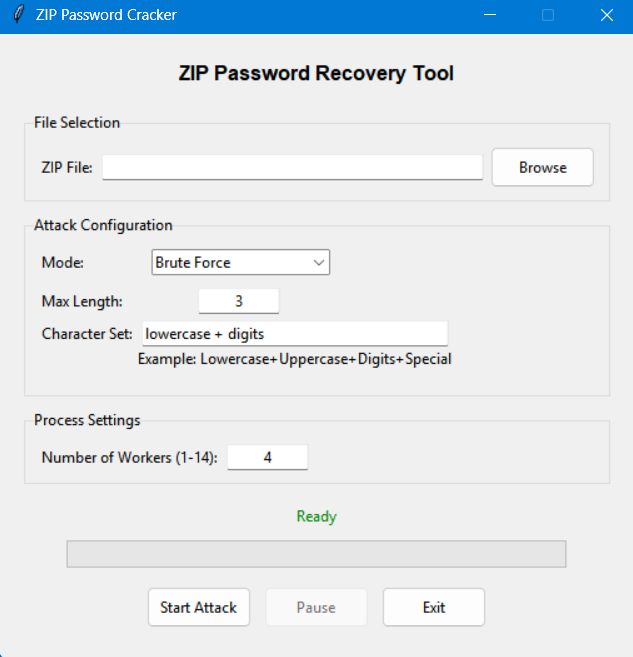
\includegraphics[width=\textwidth]{Hinhanh/GUIBruteForce.png} % Chèn hình ảnh đầu tiên
    \captionof{figure}{GUI Brute Force}
\end{minipage}
\hfill % Tạo khoảng cách giữa hai khối
\begin{minipage}[t]{0.45\textwidth}
    \centering
    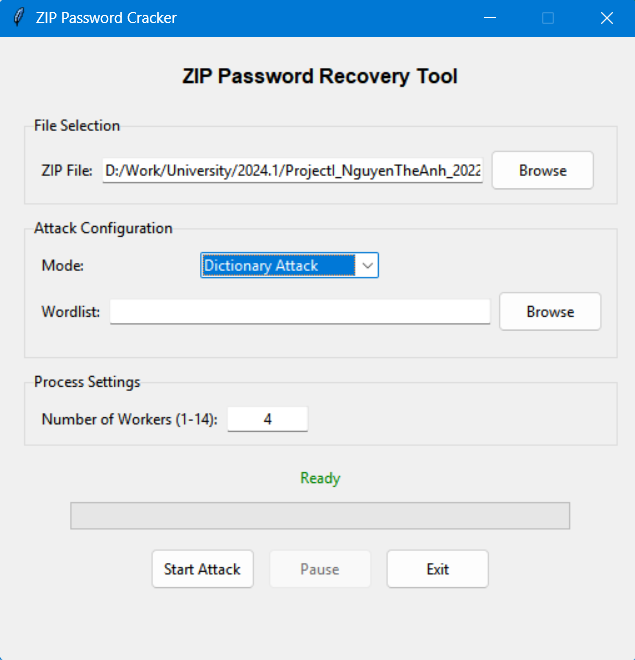
\includegraphics[width=\textwidth]{Hinhanh/GUIDictionaryAttack.png} % Chèn hình ảnh thứ hai
    \captionof{figure}{GUI Dictionary Attack}
\end{minipage}

Khi chương trình bắt đầu thực hiện tấn công, thanh tiến trình được cập nhật để hiển thị tiến độ và thời gian dự kiến. Thông báo kết thúc sẽ được gửi tới người dùng khi chương trình tìm thấy mật khẩu hoặc khi tấn công mọi tổ hợp nhưng không tìm thấy mật khẩu đúng.

\begin{minipage}[t]{0.45\textwidth}
    \centering
    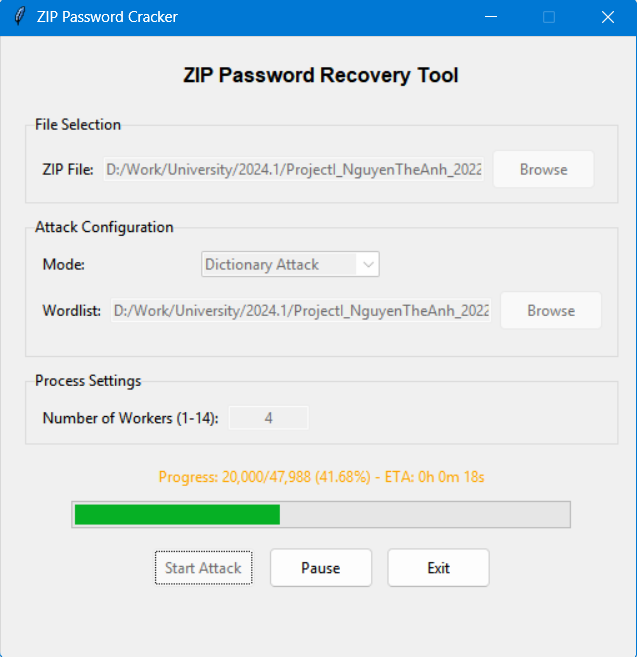
\includegraphics[width=\textwidth]{Hinhanh/Running.png} % Chèn hình ảnh đầu tiên
    \captionof{figure}{Đang tấn công}
\end{minipage}
\hfill % Tạo khoảng cách giữa hai khối
\begin{minipage}[t]{0.45\textwidth}
    \centering
    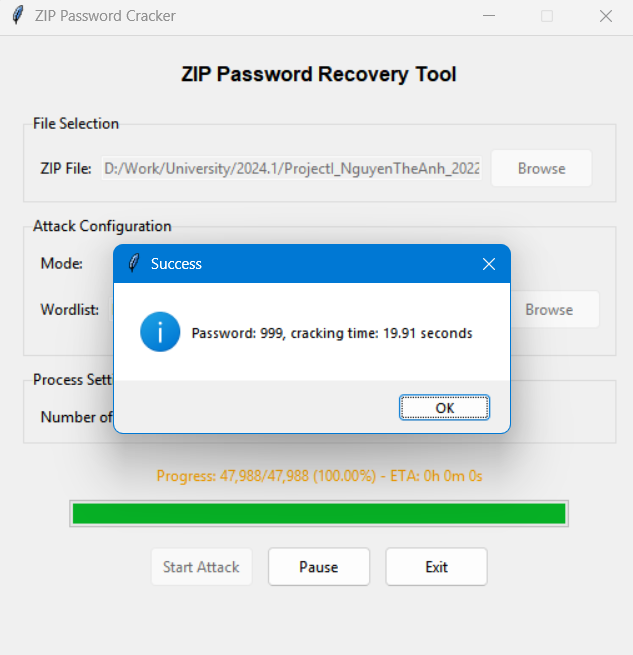
\includegraphics[width=\textwidth]{Hinhanh/Successful.png} % Chèn hình ảnh thứ hai
    \captionof{figure}{Thông báo thành công}
\end{minipage}

\end{document}
